
\section{Performance Discussions}

%We evaluated the performance of Shark and compared it with that of Hive using the TPC-H benchmark \cite{tpch} using 100GB of data on an 11-node cluster. TPC-H is the industry standard decision support benchmark, illustrating decision support systems that examine large volume of data and give answers to critical business questions.

%TPC-H is the industry standard decision support benchmark, illustrating decision support systems that examine large volume of data and give answers to critical business questions.

We evaluated the performance of Shark and compared it with that of Hive using the Brown benchmark using 72GB of data on an 11-node cluster. The benchmark was used in \cite{pavlo2009comparison} to compare the performance of Apache Hadoop versus relational database systems for large scale data processing.


\subsection{Cluster Configuration}
We used a cluster of 11 nodes on Amazon EC2 in the us-east-1b availability zone. Our experiments used High-Memory Double Extra Large Instance (m2.2xlarge) nodes with 4 cores and 34 GB of RAM. These nodes offer large memory sizes for database and memory caching applications. We used HDFS for persistent storage, with block size set to 128 MB and replication set to 3. Before each job, we cleared OS buffer caches across the cluster to measure disk read times accurately.


\subsection{Data and Queries}

\eat{
\begin{table}
	\centering
	\begin{tabular}{| l || r | r |}
		Table & File Size & Cardinality \\
		\hline
		supplier & 137M & 1M \\
		region & 389B & 5 \\
		part & 2.3G & 20M \\
		partsupp & 12G & 80M \\
		orders & 17G & 150M \\
		nation & 2.2K & 25 \\
		lineitem & 75G & 600M \\
		customer & 2.3G & 15M
	\end{tabular}
	\caption{TPC-H Table Statistics}
	\label{tb:tpch_tables}
\end{table}
}

%We used the DBGEN program provided by TPC \cite{tpch} to generate test data. Using a scaling factor of 100, we generated 100 GB of data, consisting eight tables, as documented in \ref{tb:tpch_tables}. They were first generated locally on the cluster's master node and then copied into HDFS cluster. The generation and preparation of data took approximately four hours.

%The queries we ran were adopted from \cite{tpch-hive}, which are modified from original TPC-H queries to be compatible with HiveQL while preserving the same query semantics. These queries employ varying degrees of filtering, selection, groupbys, orderbys, and aggregations.

We used the teragen and htmlgen programs \cite{pavlo2009comparison} to generate a test dataset. Using a scaling factor of 100, we generated 72 GB of data, consisting of three tables. The tables were first generated locally on the cluster's master node and then copied to the HDFS cluster. The generation and preparation of data took approximately four hours.
%, as documented in \ref{tb:tpch_tables}. 


\subsection{Performance Comparisons}

We benchmarked Shark's performance with caching enabled for the RDDs emitted by each table scan operator. We tested three different cases: while data is being cached on the first run, after the input table is cached in memory, and without any caching. Shark performs on par with or better than Hive for all of the queries in  \cite{pavlo2009comparison} on the test dataset without caching, and has more significant improvements once input data is cached. Additionally, caching data does not have a major detrimental effect on its first run. In Figure \ref{fig:query1}, we see that Shark performs equally well as Hive on un-cached data, since its runtime is dominated by loading data from disk. 

The performance improves significantly when data is cached in memory. Figure \ref{fig:query2} demonstrates that Shark has little start-up overhead, unlike Hive, which has high latency for any job. This allows Shark to provide more realtime results unlike Hive, which is realistic primarily for batch jobs. The aggregation query, Figure \ref{fig:query3}, shows similar performance on un-cached data and improvements once data is cached. The improvements due to caching are not as significant as in Query 1 or Query 2 because Shark is still limited by the shuffle phase, which requires all data to be written to disk. Finally, Figure \ref{fig:query4} shows that Shark has performance benefits for joins, primarily because Shark uses hash joins while Hive relies on Hadoop's sort-merge joins.

Since only table scan RDDs were cached in our tests, Shark's performance across first and second runs of a given query corresponds to the benefit from caching tables for queries of the same type, rather than to simply caching the final result of a query. For example, consider Query 2, which features selection and filtering. After running the query on Shark for the first time, the table data was cached in memory. Running the query for the second time benefitted from having the table data already in memory, but selection and filtering still had to be applied to the cached table data. We would expect similar performance to the second run when running a slightly different query instead, \eg selecting and filtering on different criteria. 

We would observe similar caching benefits from running the queries successively in a single Shark session. Suppose that queries 1-4 were run in succession on Shark, starting with Query 4. This query, which features a join and aggregation across the three tables would load the table data into memory, and would have an execution time of 164 seconds (1st run). Queries 3, 2, and 1 would already have their tables in memory, so their execution time would be 157, 0.7, and 6 seconds respectively (corresponding to 2nd run times), for a total of 327.7 seconds. Hive, on the other hand, would take the sum of its original execution times, or a total of 592 seconds to execute the same queries.



\begin{figure}
	\centering
	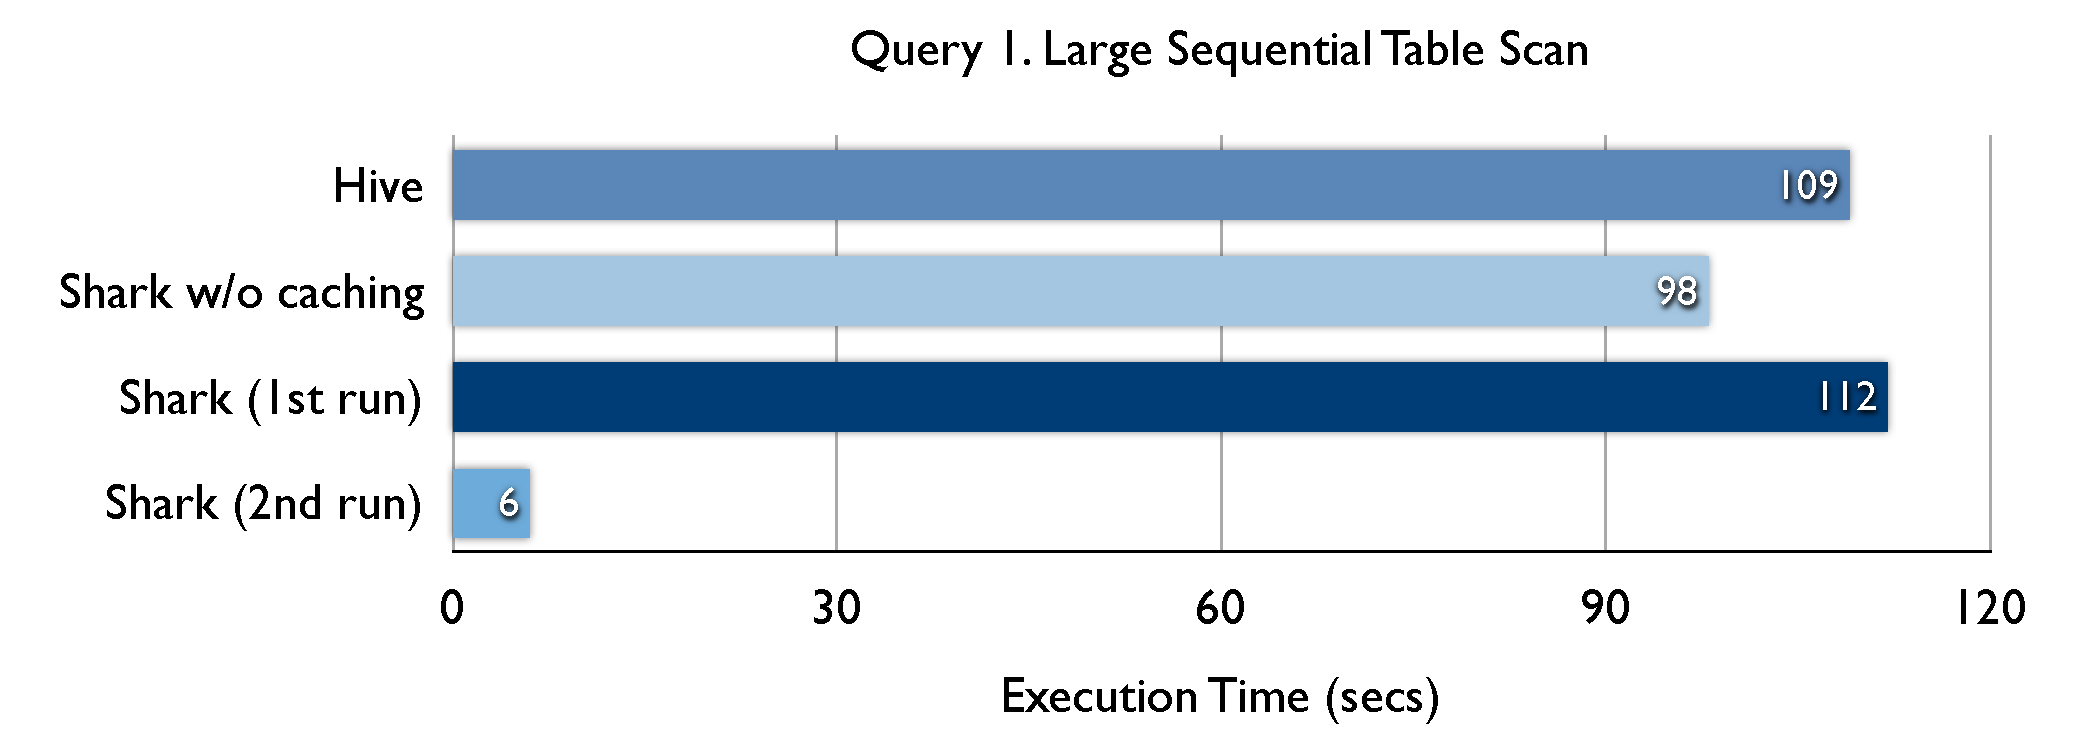
\includegraphics[width=\linewidth]{files/query1.pdf}
	\caption{Query 1 large sequential scan and grep}
	\label{fig:query1}
\end{figure}

\begin{figure}
	\centering
	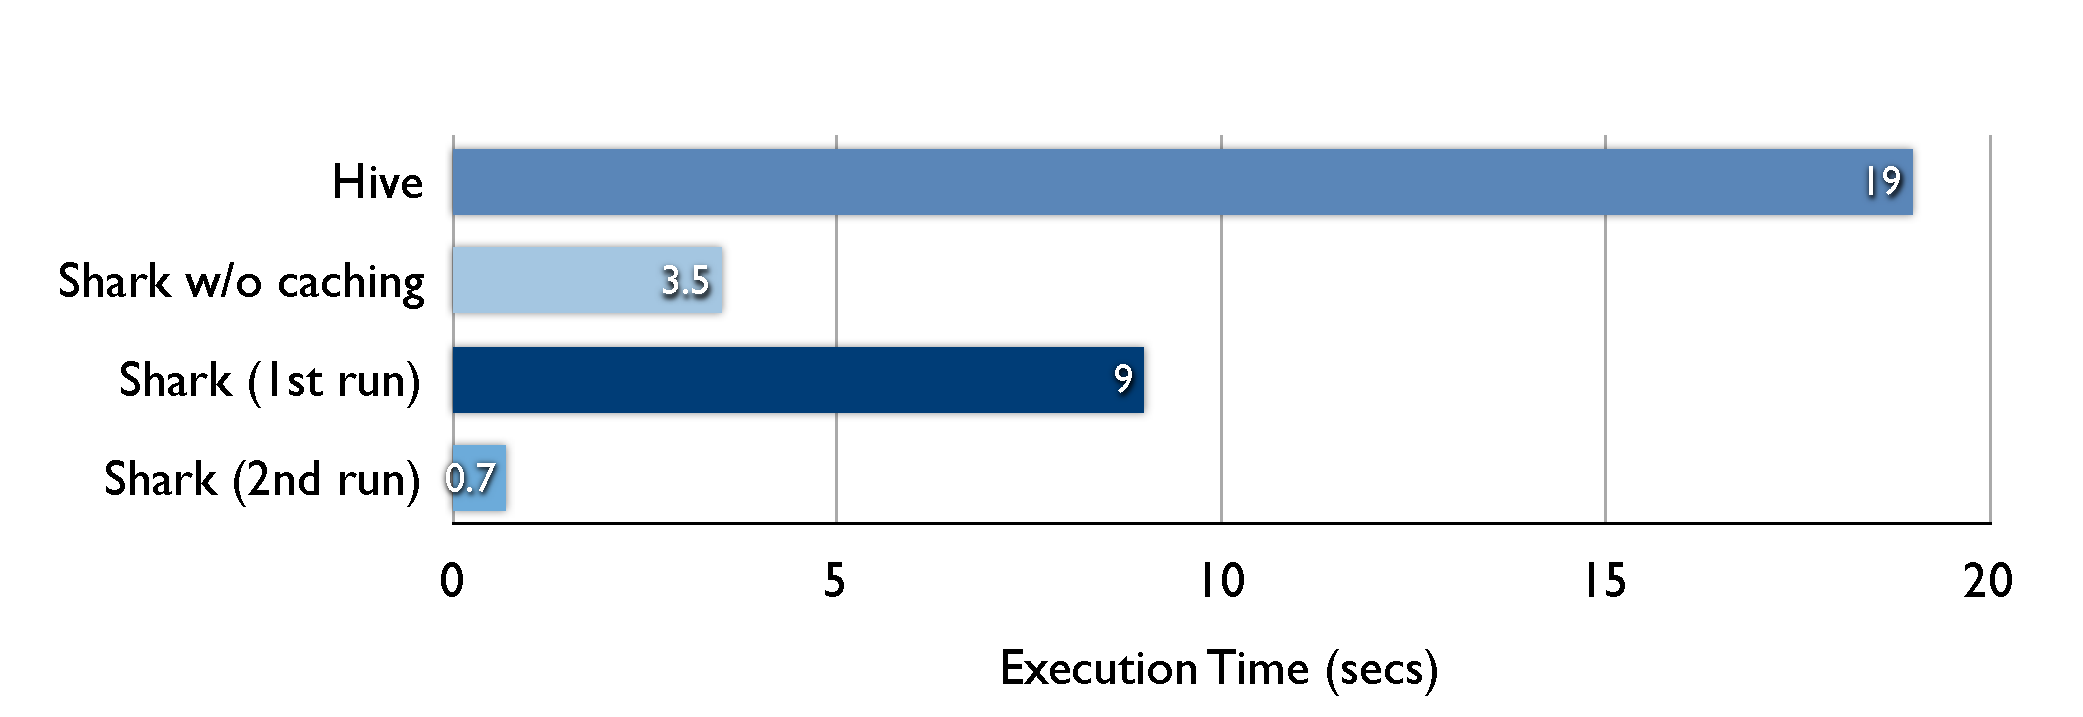
\includegraphics[width=\linewidth]{files/query2.pdf}
	\caption{Query 2 selection and filtering}
	\label{fig:query2}
\end{figure}

\begin{figure}
	\centering
	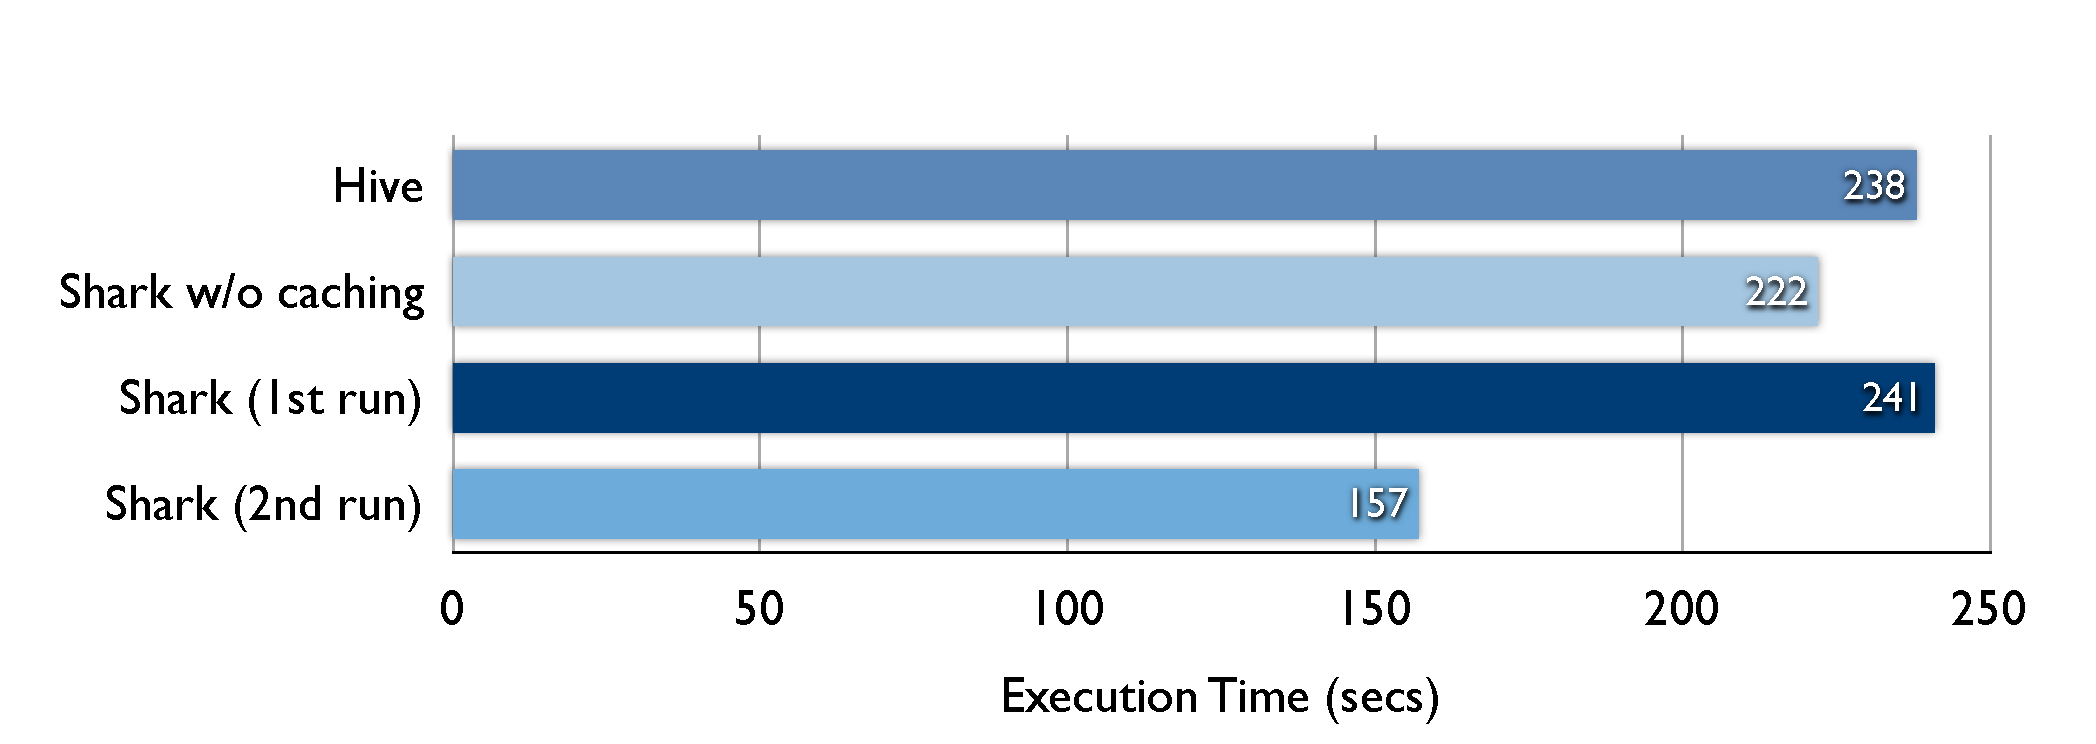
\includegraphics[width=\linewidth]{files/query3.pdf}
	\caption{Query 3 aggregation}
	\label{fig:query3}
\end{figure}

\begin{figure}
	\centering
	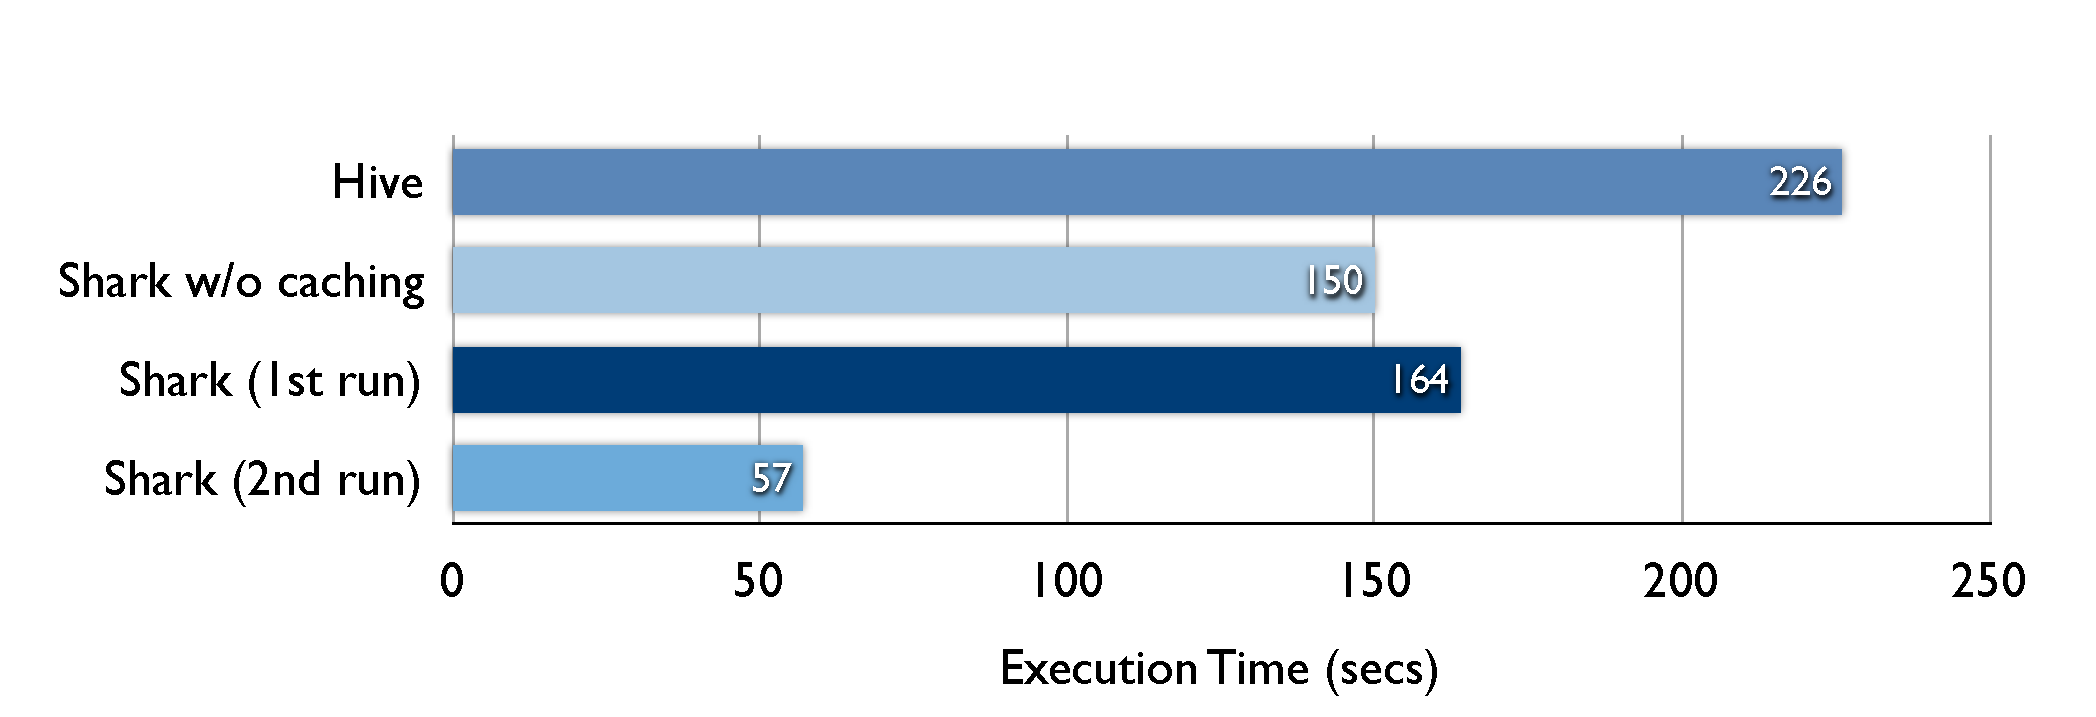
\includegraphics[width=\linewidth]{files/query4.pdf}
	\caption{Query 4 join and aggregation}
	\label{fig:query4}
\end{figure}


\subsection{JVM Memory Management}

\begin{figure}
	\centering
	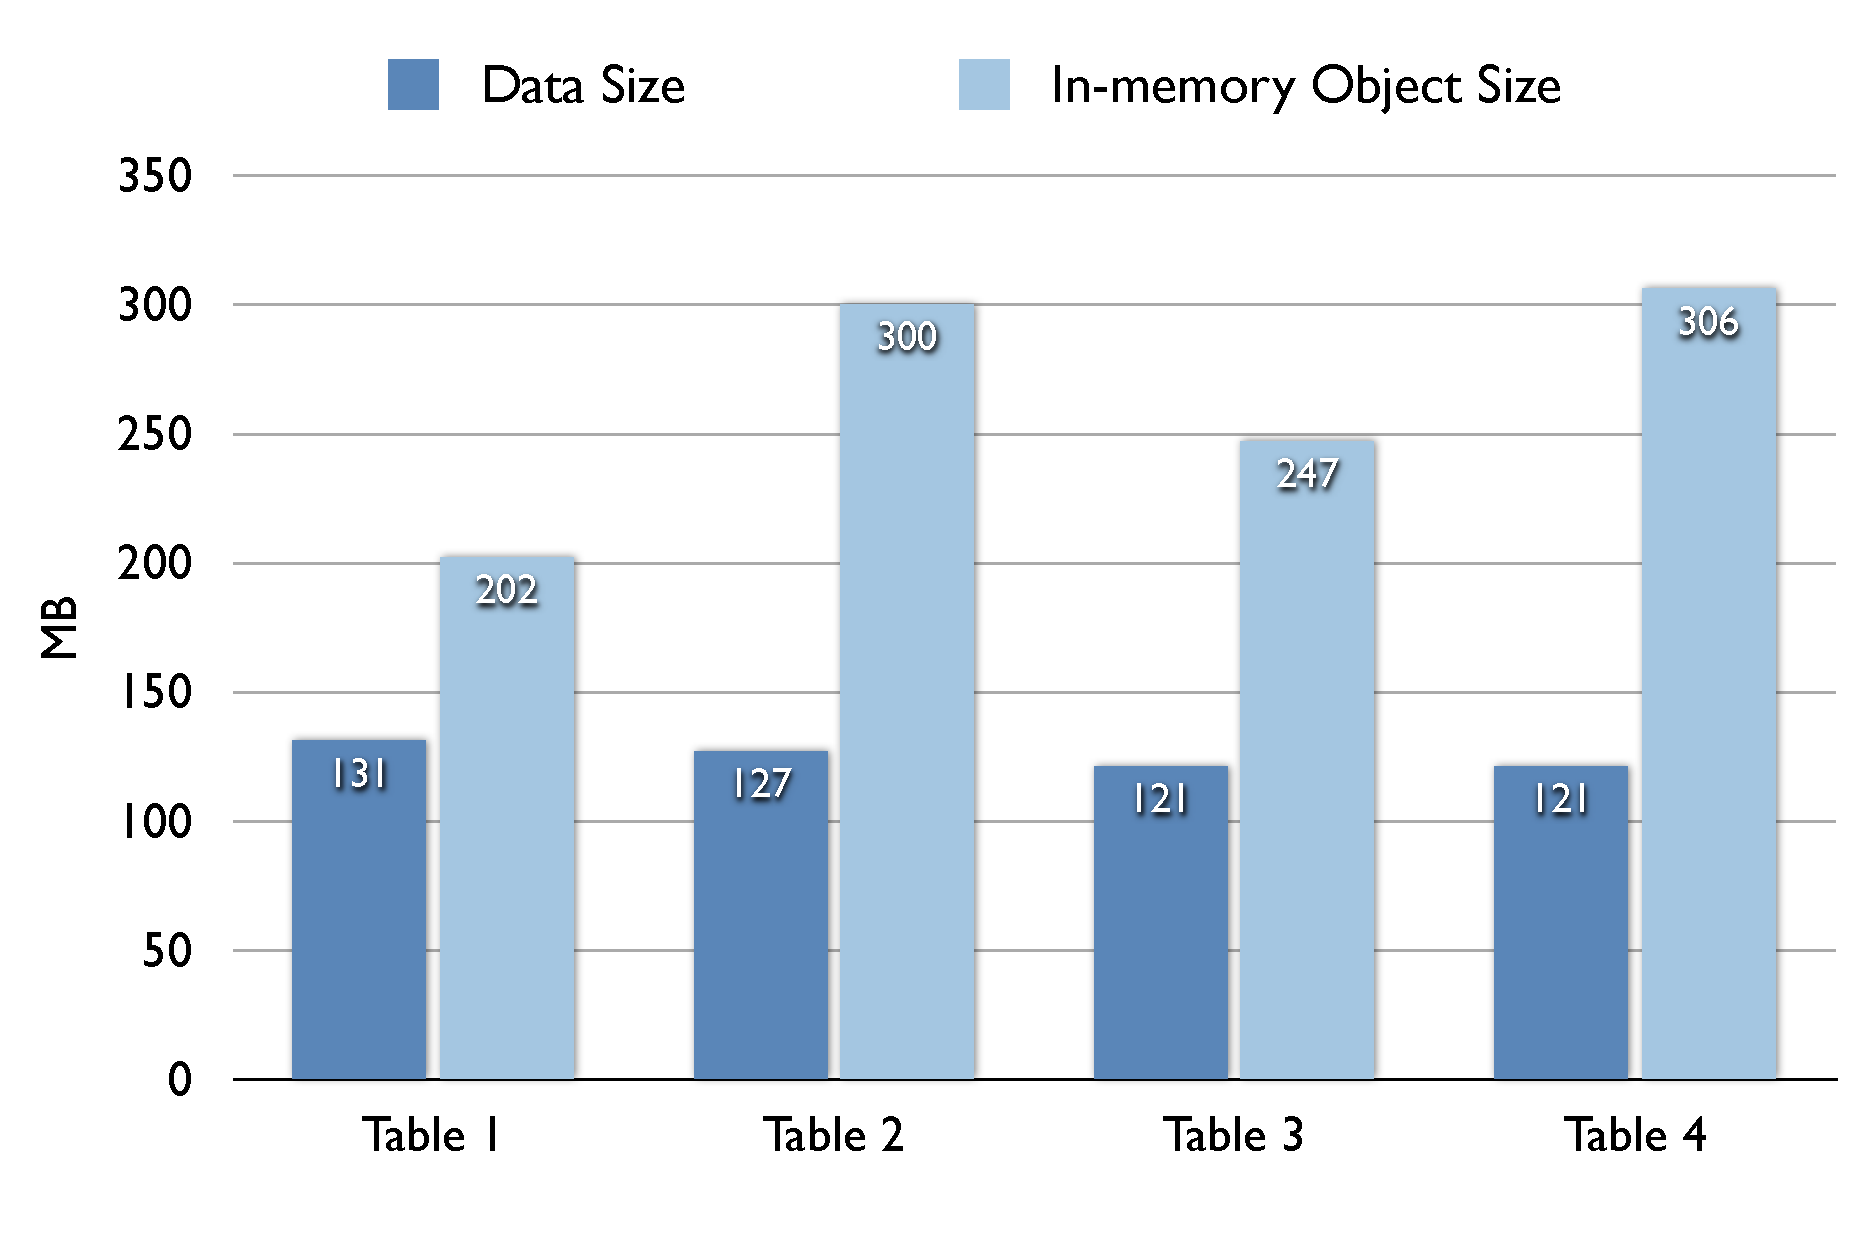
\includegraphics[width=\linewidth]{files/object-overhead.pdf}
	\caption{In-memory Java Object Overhead}
\end{figure}

Just like other programs running on top of the JVM, Shark's memory allocation and collection are managed by the JVM. There are two problems with caching large amounts of data in JVM heap. First, Cached data are considered long-lived and during their life span, they will be copied at least three times, from the eden space to the first survivor space, then to the second survivor space, and eventually to the tenured space \cite{jvm-gc}. When the long-lived data are large in size, it takes considerably large amount of time to copy the data multiple times. Second, with a very large heap, full garbage collection takes a significant chunk of time while pausing the program. Shark uses certain parts of Hive code that frequently allocates large short-lived objects. In the face of memory pressure exerted by the large data caches, these objects lead to frequent garbage collections.

The generational garbage collection is not very efficient in these cases. When we benchmarked TPC-H on Shark, with a 25GB of JVM heap space per node, normal garbage collection would take 1 - 2 seconds, while a full garbage collection would take as long as 50 seconds. When the memory usage was very high, over 90\% of the query execution time was spent in garbage collection.

This made the initial version of Shark unusable for real big data applications. We are currently studying various techniques to mitigate the problem \cite{hbase-gc}, but seem to have resolved most of these effects by implementing lazy deserialization. Our lazy deserialization dramatically improved perfomance on many of these issues by leaving deserialized rows in their original byte array format rather than converting them to Java objects. We stream the byte array through our operators and evaluate fields only when requested. Additionally, we take advantage of Spark's iterator pipelining so that we only need to keep a reference to a single byte array at a time. This allows previously used byte arrays to be garbage collected much earlier.
% add more recent performance info

%\subsection{Conviva Data Warehouse}

%Conviva Inc, a video distribution company, runs a 20 node Hive warehouse for data analytics. They have two types of queries: predefined reporting queries and ad-hoc debugging queries. 

%Their reporting queries mostly work on the same subset of the data (records matching a customer-provided predicate), but perform aggregations (averages, percentiles, and {\small\tt COUNT DISTINCT}) over different grouping fields, requiring separate MapReduce jobs. A typical reporting query takes 20 hours to run on 200 GB of compressed data. They experimented with an earlier prototype of Shark that required the developers to hand code the query plans. The query now runs in 30 mins using only two nodes with 96GB of RAM, i.e. a $40\times$ improvement in query runtime and using only 10\% of the hardware resources. The speedup comes from a combination of keeping the columns of interest in memory and avoiding repeated decompression and filtering of the same data files.

%Conviva is now running approximately 30\% of its reporting queries on the earlier prototype of Shark instead of Hive, but this requires manual porting of SQL queries. With the new version, Conviva doesn't need to rewrite their queries and will be able to achieve the same performance gains.

%In addition, a number of users at Conviva use Hive interactively for debugging \eg finding commonalities between users who experienced low video quality to identify misconfigurations and software bugs. Like the reporting queries, these queries repeatedly access and refine the same dataset, so running them over Shark would greatly reduce debug cycles.


